\documentclass[11pt,a4paper,openany]{book}
\usepackage[margin=24mm]{geometry}
\usepackage{fontspec}
\IfFontExistsTF{Noto Serif}{\setmainfont{Noto Serif}}{\setmainfont{DejaVu Serif}}
\usepackage{amsmath,amssymb,tikz,enumitem,microtype}
\usepackage[hidelinks]{hyperref}
\setlength{\parindent}{0pt}
\setlength{\parskip}{6pt}
\setlist[enumerate]{leftmargin=*,itemsep=8pt}
\setlength{\emergencystretch}{2em}

\renewcommand{\contentsname}{Mục lục}
\begin{document}
\title{V-TALENT 2045\\ PHY101-B --- Hình học, lượng giác và đồ thị\\\large Level 1 \textbar{} Mathematics for Physics}
\author{Dr. Dang Minh Tuan -- TS. Đặng Minh Tuấn}
\date{2026 \textbar{} Draft v1.0}
\maketitle
\tableofcontents
\chapter*{Hướng dẫn học}
Lớp 8–9. Tiên quyết: PHY101-A, hình học và đại số cơ bản. Dùng độ nếu không quy định khác; không cần giải tích.

Dự đoán trước; vẽ mô hình; tự tái lập ví dụ; giải độc lập và kiểm tra lời giải cuối sách. Nội dung tự biên soạn; nguồn chỉ dẫn đọc, không sao chép. Bản thảo chờ thẩm định độc lập.
\chapter{Đồng dạng và hình học quang học}
\section{Mục tiêu năng lực}
Dùng tam giác đồng dạng để suy khoảng cách không đo trực tiếp; phân biệt mô hình tia với ảnh thực.
\section{Lý thuyết và suy dẫn}
Hai tam giác có các góc tương ứng bằng nhau thì đồng dạng; tỉ số các cạnh tương ứng bằng nhau. Vẽ hình trước khi lập tỉ số, ghi rõ cạnh tương ứng và dùng cùng đơn vị. Với vật thẳng đứng cao H trên mặt phẳng ngang, bóng dài S; cọc chuẩn cao h có bóng s cùng thời điểm cho $H/S=h/s$ khi tia sáng gần song song. Đèn gần thường không thỏa mô hình tia song song.

Trong camera lỗ kim, tia thẳng qua lỗ nhỏ nối đỉnh vật với đáy màn. Tam giác đồng dạng cho $|h_i|/h_o=d_i/d_o$, các khoảng cách là độ lớn dương tính từ lỗ. Theo quy ước chiều cao có dấu, $h_i/h_o=-d_i/d_o$. Đây là phép chiếu hình học, không phải công thức thấu kính mỏng. Lỗ có kích thước hữu hạn gây nhòe; nhiễu xạ cũng giới hạn độ phân giải khi lỗ quá nhỏ.

Phản xạ ở gương phẳng tuân theo hai góc bằng nhau đo từ pháp tuyến, không phải mặt gương. Ảnh ảo ở sau gương cách gương bằng khoảng cách vật đến gương. Dựng đường thẳng biểu kiến tới ảnh; giao điểm với gương cho điểm phản xạ. Phép dựng giả sử gương phẳng và tia không bị chắn.
\begin{center}
\begin{tikzpicture}[scale=.85]\draw[dashed](-4,0)--(3,0);\draw[->,thick](-3,0)--(-3,2)node[above]{$h_o$};\draw[thick](0,-2)--(0,-.08)(0,.08)--(0,2);\draw[thick](2,-2)--(2,2);\draw[blue](-3,2)--(2,-1.333);\draw[->,thick](2,0)--(2,-1.333)node[below]{$h_i$};\node at(-1.5,-.3){$d_o$};\node at(1,.3){$d_i$};\end{tikzpicture}
\end{center}
\section{Ví dụ có lời giải}
\subsection*{Ví dụ 1.1}
Cọc 1,2 m có bóng 0,8 m; cây có bóng 7,6 m cùng thời điểm. Tìm chiều cao.

\textbf{Lời giải.} $H/7{,}6=1{,}2/0{,}8$, nên $H=11{,}4$ m. Giả sử đất ngang và tia song song.
\subsection*{Ví dụ 1.2}
Vật cao 1,8 m cách lỗ kim 6 m. Màn cách lỗ 40 mm phía sau. Tính chiều cao ảnh.

\textbf{Lời giải.} $d_i=0{,}040$ m. $h_i=-1{,}8(0{,}040)/6=-0{,}012$ m, tức ảnh ngược cao 12 mm.
\section{Nhiệm vụ thực nghiệm}
Làm camera lỗ kim bằng giấy quan sát vật trong nhà đủ sáng (không nhìn Mặt Trời). Đo ảnh ở hai khoảng cách màn, dự đoán tỉ số và thảo luận độ nhòe.
\section{Ứng dụng hiện đại và chuyển giao}
Camera đã hiệu chuẩn đơn giản có khoảng cách chiếu hiệu dụng 5 mm. Vật chuẩn 0,6 m tạo ảnh 1,5 mm, suy khoảng cách 2 m. Đây là cơ sở ước lượng khoảng cách bằng thị giác máy khi biết kích thước và hướng vật. Camera thật cần hiệu chuẩn thấu kính và hiệu chỉnh méo.
\section{Chỉ dẫn đọc nguồn}
SJ ch. 29 (geometric optics), p. 106; source catalogue SJ-29; optical reading is an extension.
\section{Luyện tập độc lập}
\begin{enumerate}
\item \textbf{PHY101-B-1.1}. Cọc 1,5 m có bóng 2 m; tháp có bóng 18 m. Tìm chiều cao tháp.
\item \textbf{PHY101-B-1.2}. Ảnh lỗ kim của vật 30 cm ở xa 2 m cao 6 mm. Tìm khoảng cách màn.
\item \textbf{PHY101-B-1.3}. Tia hợp mặt gương phẳng 25 độ. Tìm góc tới và phản xạ.
\item \textbf{PHY101-B-1.4}. Đèn cao 3 m, cọc cao 1 m cách chân đèn 2 m theo phương ngang. Tìm chiều dài bóng kể từ chân cọc trên đất ngang.
\end{enumerate}
\chapter{Lượng giác, vector và dẫn đường}
\section{Mục tiêu năng lực}
Phân tích vector theo hai phương vuông góc; khôi phục độ lớn và hướng; dùng bất đẳng thức tam giác.
\section{Lý thuyết và suy dẫn}
Với tam giác vuông cạnh huyền c, góc $\theta$, $\sin\theta=\text{đối}/c$, $\cos\theta=\text{kề}/c$, $\tan\theta=\text{đối}/\text{kề}$. Pythagoras cho $\sin^2\theta+\cos^2\theta=1$. Vector độ lớn A hợp góc $\theta$ ngược chiều kim đồng hồ từ x dương có thành phần $A_x=A\cos\theta$, $A_y=A\sin\theta$. Thành phần có thể âm; độ lớn không âm.

Cộng vector bằng quy tắc nối đuôi–đầu hoặc cộng thành phần tương ứng. Độ lớn tổng $\sqrt{R_x^2+R_y^2}$. Với hai vector độ lớn a,b, $|a-b|\le R\le a+b$, dấu bằng khi cùng phương. Tỉ số tang không tự xác định góc phần tư. Ví dụ cả hai thành phần âm thì vector ở góc phần tư III dù tỉ số tang dương. Góc phương vị thường đo theo chiều kim đồng hồ từ Bắc, khác góc toán học.

Trong dòng chảy đều, vận tốc so với đất bằng tổng vector vận tốc thuyền so với nước và dòng. Muốn qua sông vuông góc bờ, thành phần ngược dòng phải bù dòng. Không thể qua đúng điểm đối diện nếu dòng nhanh bằng hoặc hơn thuyền (bằng nhau thì thành phần ngang sông bằng 0). Qua nhanh nhất lại cần cực đại thành phần ngang và có thể bị trôi.
\begin{center}
\begin{tikzpicture}[scale=.8]\draw[->](0,0)--(5,0)node[right]{$x$};\draw[->](0,0)--(0,4)node[above]{$y$};\draw[->,very thick,blue](0,0)--(4,3)node[above]{$\vec A$};\draw[dashed](4,3)--(4,0);\node at(2,-.3){$A_x$};\node[right]at(4,1.5){$A_y$};\draw(1,0)arc(0:36.87:1);\end{tikzpicture}
\end{center}
\section{Ví dụ có lời giải}
\subsection*{Ví dụ 2.1}
Lực 10 N hướng 30 độ lên trên phương ngang. Tìm thành phần.

\textbf{Lời giải.} $F_x=10\cos30^\circ=5\sqrt3\approx8{,}66$ N; $F_y=10\sin30^\circ=5$ N.
\subsection*{Ví dụ 2.2}
Drone bay 3 km về Đông rồi 4 km về Bắc. Tìm độ lớn và hướng độ dời.

\textbf{Lời giải.} $R=\sqrt{3^2+4^2}=5$ km; góc từ Đông về Bắc $\arctan(4/3)\approx53{,}13^\circ$. Quãng đường 7 km.
\section{Nhiệm vụ thực nghiệm}
Dùng giấy ô ly cộng hai vector độ dời ở các góc khác nhau. Đo độ lớn tổng và đối chiếu tính thành phần. Thảo luận sai số đọc tỉ lệ.
\section{Ứng dụng hiện đại và chuyển giao}
Robot di động ước lượng 1,2 m về Đông và 0,5 m về Bắc từ bánh xe. Độ dời thẳng 1,3 m. Nếu bánh trượt, ước lượng thành phần bị lệch; mốc thị giác độc lập có thể hiệu chỉnh.
\section{Chỉ dẫn đọc nguồn}
SJ §§5.1–5.2, pp. 20–23 (vector concepts; defer calculus and cross product).
\section{Luyện tập độc lập}
\begin{enumerate}
\item \textbf{PHY101-B-2.1}. Phân tích lực 20 N hợp 60 độ phía trên +x.
\item \textbf{PHY101-B-2.2}. Cộng vector (-3,4) và (5,-1) theo mét; tìm độ lớn.
\item \textbf{PHY101-B-2.3}. Thuyền đi 5 m/s so với nước; dòng 3 m/s. Tìm tốc độ ngang khi hướng tới điểm đối diện.
\item \textbf{PHY101-B-2.4}. Hai lực có độ lớn 6 N và 8 N. Hợp lực có thể là 1 N? 10 N? Giải thích.
\end{enumerate}
\chapter{Đồ thị, độ dốc và đại lượng tích lũy}
\section{Mục tiêu năng lực}
Đọc trục và đơn vị, phân biệt độ dốc với độ cao, tìm diện tích đại số bằng hình học.
\section{Lý thuyết và suy dẫn}
Đồ thị biểu diễn cặp giá trị, không phải hình đường đi thật. Ghi đại lượng và đơn vị mỗi trục. Đoạn thẳng có độ dốc $\Delta y/\Delta x$ phụ thuộc hai trục. Đồ thị x–t có độ dốc là vận tốc; v–t có độ dốc là gia tốc. Giao trục biểu thị giá trị đầu hay độ lệch, không mặc nhiên là sai số. Độ dốc nhìn bằng mắt phụ thuộc tỉ lệ trục nên phải tính.

Vận tốc không đổi cho độ dời bằng diện tích chữ nhật $v\Delta t$. Vận tốc biến thiên tuyến tính cho diện tích đại số hình thang $(v_1+v_2)\Delta t/2$. Nếu vận tốc qua 0, chia khoảng tại đó: diện tích đại số cho độ dời, tổng trị tuyệt đối cho quãng đường. Tương tự diện tích công suất–thời gian cho năng lượng với công suất hằng hay tuyến tính từng đoạn. Kiểm tra tích đơn vị hai trục.

Mô hình tuyến tính $y=ax+b$ cần kiểm tra với nhiều phép đo. Vẽ đường xu hướng, không ép qua gốc nếu vật lý và dữ liệu không đòi hỏi. Chọn hai điểm cách xa trên đường khớp để tính độ dốc; không nối dao động nhiễu như thể mọi biến thiên là định luật. Đồ thị có thể ủng hộ mô hình trong miền đo, không chứng minh ngoài miền.
\begin{center}
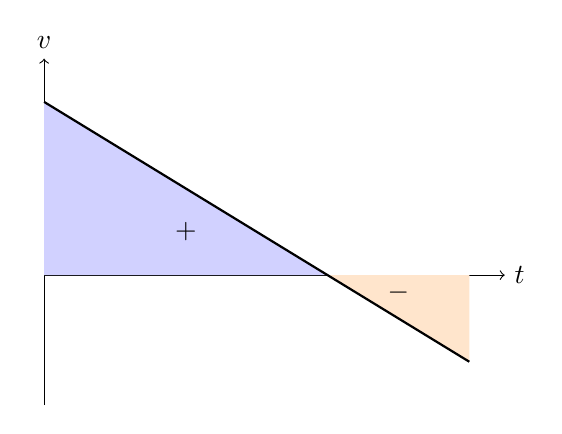
\begin{tikzpicture}[x=.9cm,y=.55cm]\draw[->](0,0)--(6.5,0)node[right]{$t$};\draw[->](0,-3)--(0,5)node[above]{$v$};\fill[blue!18](0,0)--(0,4)--(4,0)--cycle;\fill[orange!20](4,0)--(6,-2)--(6,0)--cycle;\draw[thick](0,4)--(6,-2);\node at(2,1){$+$};\node at(5,-.4){$-$};\end{tikzpicture}
\end{center}
\section{Ví dụ có lời giải}
\subsection*{Ví dụ 3.1}
Vận tốc giảm đều từ 4 đến -2 m/s trong 6 s. Tìm gia tốc, độ dời, quãng đường.

\textbf{Lời giải.} $a=(-2-4)/6=-1$ m/s$^2$. Qua 0 tại 4 s. Diện tích dương 8 m, âm -2 m: độ dời 6 m, quãng đường 10 m.
\subsection*{Ví dụ 3.2}
Thiết bị dùng 20 W trong 10 s rồi công suất tăng đều từ 20 đến 60 W trong 5 s. Tìm năng lượng.

\textbf{Lời giải.} $E=20(10)+(20+60)5/2=400$ J.
\section{Nhiệm vụ thực nghiệm}
Quay video xe đồ chơi, ghi vị trí cách đều thời gian, vẽ x theo t và ước lượng độ dốc. So sánh các đoạn thay vì giả định tốc độ đều.
\section{Ứng dụng hiện đại và chuyển giao}
Bộ ghi pin đo công suất theo thời gian. Cộng diện tích hình thang ước lượng năng lượng, hữu ích khi thiết kế thiết bị di động. Lấy mẫu thưa có thể bỏ qua đỉnh nhanh; so sánh khoảng lấy mẫu trước khi lập dự toán năng lượng.
\section{Chỉ dẫn đọc nguồn}
SJ §§4.2–4.3, pp. 15–16; SW graph reading locator from catalogue (not rechecked).
\section{Luyện tập độc lập}
\begin{enumerate}
\item \textbf{PHY101-B-3.1}. Tọa độ tăng từ 2 m lên 14 m trong 3 s trên đoạn thẳng x–t. Tìm vận tốc.
\item \textbf{PHY101-B-3.2}. Vận tốc 3 m/s trong 4 s rồi -2 m/s trong 3 s. Tìm độ dời, quãng đường.
\item \textbf{PHY101-B-3.3}. Đồ thị U–I tuyến tính qua (0,1 A;2 V) và (0,3 A;6 V). Tìm độ dốc và giao trục.
\item \textbf{PHY101-B-3.4}. Đèn 100 W hoạt động 15 phút. Biểu diễn năng lượng theo J và Wh.
\end{enumerate}
\chapter{Tối ưu hình học và chuyển giao mô hình}
\section{Mục tiêu năng lực}
Tối ưu khoảng cách và diện tích đơn giản bằng hình học; phân biệt tối ưu toán với tối ưu vật lý có ràng buộc.
\section{Lý thuyết và suy dẫn}
Bất đẳng thức tam giác cho đường thẳng ngắn nhất giữa hai điểm trong mặt phẳng Euclid không vật cản. Với tuyến A đến B chạm đường gương, phản xạ B qua gương thành B'. Mọi điểm P trên gương có $AP+PB=AP+PB'\ge AB'$. Dấu bằng khi P nằm trên đoạn AB'. Kiểm tra đoạn gương cho phép có chứa P. Kết quả chỉ tối thiểu thời gian nếu tốc độ hai chặng như nhau.

Hình chữ nhật chu vi cố định 2S có diện tích $A=x(S-x)=S^2/4-(x-S/2)^2$ lớn nhất tại $x=S/2$. Hình vuông tối ưu vì bình phương bị trừ không âm. Nếu có bề rộng tối thiểu, ràng buộc vật liệu hay chi phí cạnh khác nhau thì miền khả thi hoặc hàm mục tiêu thay đổi. Không áp dụng tối ưu không ràng buộc một cách máy móc.

Với lực độ lớn F và độ dời s cố định, công $W=Fs\cos\theta$ cực đại khi lực cùng hướng độ dời. Nhưng nếu lực kéo làm đổi phản lực thì ma sát cũng đổi: công lực kéo cực đại chưa chắc gia tốc tổng cực đại. Phân biệt này dẫn tới động lực học liên kết ở PHY202-A.
\begin{center}
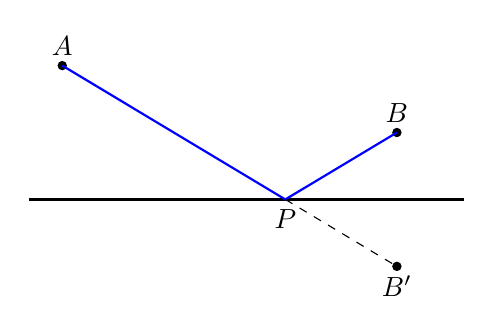
\begin{tikzpicture}[scale=.85]\draw[thick](-.5,0)--(6,0);\fill(0,2)circle(2pt)node[above]{$A$};\fill(5,1)circle(2pt)node[above]{$B$};\fill(5,-1)circle(2pt)node[below]{$B'$};\draw[blue,thick](0,2)--(3.333,0)--(5,1);\draw[dashed](3.333,0)--(5,-1);\node[below]at(3.333,0){$P$};\end{tikzpicture}
\end{center}
\section{Ví dụ có lời giải}
\subsection*{Ví dụ 4.1}
A=(0,2), B=(6,1) mét, gương y=0. Tìm đường phản xạ ngắn nhất và điểm phản xạ.

\textbf{Lời giải.} $B'=(6,-1)$. Đường A đến B' gặp y=0 tại tỉ phần $2/3$, nên $P=(4,0)$. Chiều dài $\sqrt{6^2+3^2}=3\sqrt5$ m.
\subsection*{Ví dụ 4.2}
Khung cảm biến chữ nhật chu vi 40 cm. Tối đa diện tích; sau đó thêm chiều rộng không quá 6 cm.

\textbf{Lời giải.} $A=x(20-x)=100-(x-10)^2$. Không ràng buộc: 10 x 10 cm, 100 cm$^2$. Với $0<x\le6$, gần 10 nhất là x=6; diện tích $6(14)=84$ cm$^2$.
\section{Nhiệm vụ thực nghiệm}
Trên giấy ô ly phản xạ điểm qua đường và đo ba đường gấp khúc. So với phép dựng phản xạ thẳng; lặp lại với đoạn gương giới hạn.
\section{Ứng dụng hiện đại và chuyển giao}
Kính tiềm vọng và thiết bị quang gập dùng hình học gương để đổi hướng tia trong vỏ giới hạn. Mô hình đường ngắn hữu ích khi bố trí, nhưng thiết kế thực còn ràng buộc kích thước gương, căn chỉnh, trường nhìn và chất lượng ảnh.
\section{Chỉ dẫn đọc nguồn}
SJ §7.2 (range optimization), p. 29; further reading in PHY202-A and PHY205-C.
\section{Luyện tập độc lập}
\begin{enumerate}
\item \textbf{PHY101-B-4.1}. Hình chữ nhật chu vi 28 m. Tìm diện tích lớn nhất.
\item \textbf{PHY101-B-4.2}. A=(0,3), B=(8,1), gương y=0. Tìm điểm phản xạ và chiều dài.
\item \textbf{PHY101-B-4.3}. Lực 15 N dịch thùng 4 m. So sánh công với góc 0, 60, 90 độ.
\item \textbf{PHY101-B-4.4}. Vì sao tuyến ngắn nhất có thể không nhanh nhất khi đi qua hai môi trường tốc độ sóng khác nhau? Cho phản ví dụ bằng khoảng cách và tốc độ.
\end{enumerate}
\chapter*{Tài liệu và mô phỏng}
Tan Chien Hao (2024). \textit{Freshman Physics}.\par
Swiss Physics Olympiad Script, 3rd ed. (2019), catalogue locators pending recheck.\par
\url{https://www.math.ust.hk/~machas/differential-equations.pdf}\par
\url{https://diavn.github.io/truongchuyen/physics-curriculum.html}\par
\url{https://diavn.github.io/truongchuyen/physics-dynamics-lab.html}
\appendix
\chapter{Lời giải đầy đủ}
\section{Đồng dạng và hình học quang học}
\begin{enumerate}
\item \textbf{PHY101-B-1.1}. $H=18(1{,}5/2)=13{,}5$ m.
\item \textbf{PHY101-B-1.2}. $d_i=2(0{,}006/0{,}30)=0{,}040$ m.
\item \textbf{PHY101-B-1.3}. Pháp tuyến vuông góc mặt: $i=90^\circ-25^\circ=65^\circ=r$.
\item \textbf{PHY101-B-1.4}. Gọi bóng dài s. Đồng dạng cho $3/(2+s)=1/s$, nên $3s=2+s$, $s=1$ m.
\end{enumerate}
\section{Lượng giác, vector và dẫn đường}
\begin{enumerate}
\item \textbf{PHY101-B-2.1}. $F_x=10$ N; $F_y=10\sqrt3$ N.
\item \textbf{PHY101-B-2.2}. Tổng $(2,3)$ m; độ lớn $\sqrt{13}$ m.
\item \textbf{PHY101-B-2.3}. Thành phần ngược dòng 3 m/s; ngang $\sqrt{25-9}=4$ m/s.
\item \textbf{PHY101-B-2.4}. Miền 2 đến 14 N. 1 N không thể; 10 N xảy ra khi vuông góc theo Pythagoras.
\end{enumerate}
\section{Đồ thị, độ dốc và đại lượng tích lũy}
\begin{enumerate}
\item \textbf{PHY101-B-3.1}. $v=(14-2)/3=4$ m/s.
\item \textbf{PHY101-B-3.2}. Độ dời $12-6=6$ m; quãng đường $12+6=18$ m.
\item \textbf{PHY101-B-3.3}. Độ dốc $(6-2)/(0{,}3-0{,}1)=20$ V/A = 20 ohm; giao trục $2-20(0{,}1)=0$ V.
\item \textbf{PHY101-B-3.4}. $E=100(900)=90000$ J; $100(0{,}25)=25$ Wh.
\end{enumerate}
\section{Tối ưu hình học và chuyển giao mô hình}
\begin{enumerate}
\item \textbf{PHY101-B-4.1}. $A=x(14-x)=49-(x-7)^2$; cực đại 49 m$^2$ khi 7 x 7.
\item \textbf{PHY101-B-4.2}. Phản xạ B thành $(8,-1)$; tỉ phần $3/4$ cho P=(6,0); độ dài $\sqrt{64+16}=4\sqrt5$.
\item \textbf{PHY101-B-4.3}. $W=60\cos\theta$: 60 J, 30 J, 0 J. Công tổng có thể gồm lực khác.
\item \textbf{PHY101-B-4.4}. Thời gian cộng $d_i/v_i$, không cộng riêng độ dài. A: 4 m chậm ở 1 m/s và 1 m nhanh ở 5 m/s mất 4,2 s. B: 1 m chậm, 5 m nhanh mất 2 s dù dài 6 m so với 5 m. Cần kiểm tra hình học khả thi thực tế.
\end{enumerate}
\end{document}
